\chapter{Lecture 25 - Convection with Metallic Fluids}
\label{ch:ch25}
\section{Objectives}
The objectives of this lecture are:
\begin{enumerate}
\item Present correlations to characterize convective heat transfer for fully developed turbulent flow in smooth circular tubes with metallic fluids.
\item Present a correlation for convective heat transfer with metallic fluids between parallel flat plates and concentric annuli.
\item Present correlations for convective heat transfer with metallic fluids in rod bundles.
\end{enumerate}

\section{Liquid Metal Convection Correlations}
\newthought{When it comes} to convection, liquid metals are different.  The balance between conduction and advection present in all convection problems is less heavily skewed towards advection, particularly for flow conditions prevalent in liquid metal reactors---or at least liquid metal reactor design concepts.  One other difference between convection for common fluids like air or water and liquid metals is the vast disparity in operating experience and experimental results on which to base correlations.  

The basic form of Nusselt number correlations for liquid metals is shown in Equation \ref{eq:basic-lm}:

\begin{equation}
\text{Nu}_{\infty} = A + B(\text{Pe}^{C}
\label{eq:basic-lm}
\end{equation}
where $A$, $B$, and $C$ are constants that depend on the geometry  and boundary conditions---$C$ being close to 0.8 and $A$ reflecting the significance of conductive heat transfer even at low Reynolds number; and Pe is the Peclet number which is defined as the product of Reynolds number and Prandtl number.\marginnote{\textbf{Peclet number:} a dimensionless number characterizing the ratio of heat transfer by convection to the heat transfer by conduction.} \index{Peclet number}

\begin{equation}
\text{Pe} = \text{Re} \cdot \text{Pr}
\end{equation}


\section{Circular Tube Correlations}
\newthought{For circular tubes} with constant heat flux along the tube boundaries, Lyon provides a correlation \cite{lyon1951liquid} given by Equation \ref{eq:lyon}: \index{Lyon correlation}

\begin{equation}
\text{Nu}_{\infty} = 7 + 0.025 \text{Pe}^{0.8}
\label{eq:lyon}
\end{equation}

For smooth circular tubes with uniform wall temperature, a correlation is provided by Seban and Shimazaki\cite{seban1949heat} given by Equation \ref{eq:seban}: \index{Seban and Shimazaki correlation}
\begin{equation}
\text{Nu}_{\infty} = 5 + 0.025 \text{Pe}^{0.8}
\label{eq:seban}
\end{equation}

\section{Flow Past Parallel Plates and Concentric Annuli}
\newthought{For fully developed} flow with constant heat flux through one wall only, Seban provides the following correlation\cite{seban1950heat} given by Equation \ref{eq:seban2}: \index{Seban correlation, parallel plates} 

\begin{equation}
\text{Nu}_{\infty} = 5.8 + 0.02 \text{Pe}^{0.8}
\label{eq:seban2}
\end{equation}

Seban presented another correlation for fully developed flow through concentric annuli with uniform heat flux on the inner wall; this is given in Equation \ref{eq:seban3} \index{Seban correlation, concentric annuli}

\begin{equation}
\text{Nu}_{\infty} = 5.25 + 0.0188\text{Pe}^{0.8}\left(\frac{D_2}{D_1} \right)^{0.3}
\label{eq:seban3}
\end{equation}
where $D_1$ and $D_2$ are as shown in Figure \ref{fig:annuli} and $\sfrac{D_2}{D_1} > 1.4$.
\begin{marginfigure}
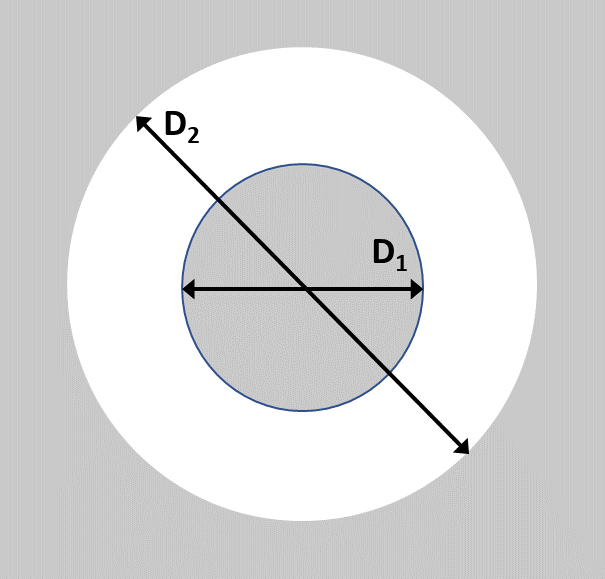
\includegraphics{concentric_annuli.png}
\caption{Concentric annuli geometry.}
\label{fig:annuli}
\end{marginfigure}
In the case that the concentric annuli are very closely fitted such that $D_2 \approx D_1$ then Seban recommends that Equation \ref{eq:seban2} be used instead.

\section{Flow in Rod Bundles}
\newthought{The course textbook} lists a few correlations that can be used for flow in rod bundles.  As one might expect from previous discussion on low in rod bundles, it is essential that some dependence on pitch-to-diameter ratio is captured as this geometric parameter has great influence on flow behavior and resultant convective heat transfer performance.

Two of the correlations presented by Kazimi and Carelli are repeated here\cite{kazami1976heat}; one we will refer to simply as the Kazimi and Carelli correlation given in Equation \ref{eq:kaz-car}; \index{Kazimi and Carelli correlation}

\begin{equation}
\text{Nu}_{\infty} = 4.0 + 0.33\left(\frac{P}{D}\right)^{3.8}\left(\frac{\text{Pe}}{100} \right)^{0.86} + 0.16 \left(\frac{P}{D}\right)^{5.0}
\label{eq:kaz-car}
\end{equation}
for $1.1 \le \sfrac{P}{D} \le 1.4$ and $10 \le \text{Pe} \le 5000$.
The other is the Schad-modified correlation given by Equation \ref{eq:schad-mod1} and Equation \ref{eq:schad-mod2}: \index{Schad-modified correlation}

\begin{equation}
\text{Nu}_{\infty} = \left[-16.15 + 24.96 \left(\frac{P}{D} \right) - 8.55 \left(\frac{P}{D} \right)^2 \right]\text{Pe}^{0.3}
\label{eq:schad-mod1}
\end{equation}
for $1.1 \le \sfrac{P}{D} \le 1.5$ and $150 \le \text{Pe} \le 1000$

\begin{equation}
\text{Nu}_{\infty} = 4.496\left[-16.15 + 24.96 \left(\frac{P}{D} \right) - 8.55 \left(\frac{P}{D} \right)^2 \right]
\label{eq:schad-mod2}
\end{equation}
for $\text{Pe} \le 150$.

Lastly, we include a correlation provided by Borishanskii et al \cite{borishanskii1969heat} which covers a similar range of $\sfrac{P}{D}$ and Peclet numbers, and is given in Equation \ref{eq:boris}: \index{Borishanskii correlation}

\begin{multline}
\text{Nu}_{\infty} = 24.15 \ln{\left[-8.12 + 12.76\left(\frac{P}{D}\right)-3.65 \left(\frac{P}{D} \right)^2  \right]} \\ + 0.0174\left[1 - e^{6 - 6\sfrac{P}{D}} \right] \left[\text{Pe} - 200 \right]^{0.9}
\label{eq:boris}
\end{multline}
for $1.1 \le \sfrac{P}{D} \le 1.5$ and $200 \le \text{Pe} \le 2000$ and if $\text{Pe}< 200$ you should omit the last part of Equation \ref{eq:boris} and just use:

\begin{equation}
\text{Nu}_{\infty} = 24.15 \ln{\left[-8.12 + 12.76\left(\frac{P}{D}\right)-3.65 \left(\frac{P}{D} \right)^2  \right]}
\end{equation}

\newthought{Right about now} the reader may be wondering: \emph{``...out of all these correlations, which one should I choose?''}.  A fair question, and my short answer is: all potentially applicable correlations. There may be some insight to be gained in comparing the results from different applicable correlations; perhaps some idea as to the uncertainty based on the range of results returned by different correlations.  That would be something, but not anything you would hang your hat on.  Whatever the result, from whichever correlation, you should understand that extensive testing---whether on prototypes or as pre-operational testing on the as-constructed system---will be required to prove that performance is within expected bounds.


